%%%%%%%%%%%%%%%%%%%%%%%%%%%%%%%%%%%%%%%%%%%%
\section{Workshops}


\begin{frame}
      \frametitle{Table of Contents}
      \tableofcontents[currentsection]
\end{frame}




%%%%%%%%%%%%%%%%%%%%%%%%%%%%%%%%%%%%%%%%%%%%%
\subsection{Four-lesson Curriculum}

%%%%%%%%%%%%%%%%%%%%%%%%%%%%%%%%%%%%%%%%%%%%%%%%%%%%%%%%
{
\paper{Badillo-Perez A, Badillo-Perez D, Barco A, Montenegro R, Xochicale M. 2013, Teaching AI and Robotics to Children in a Mexican town, DEI-HRI2023, \url{https://arxiv.org/abs/2303.03956}}

\begin{frame}{Curriculum}
      \begin{figure}
        \centering
        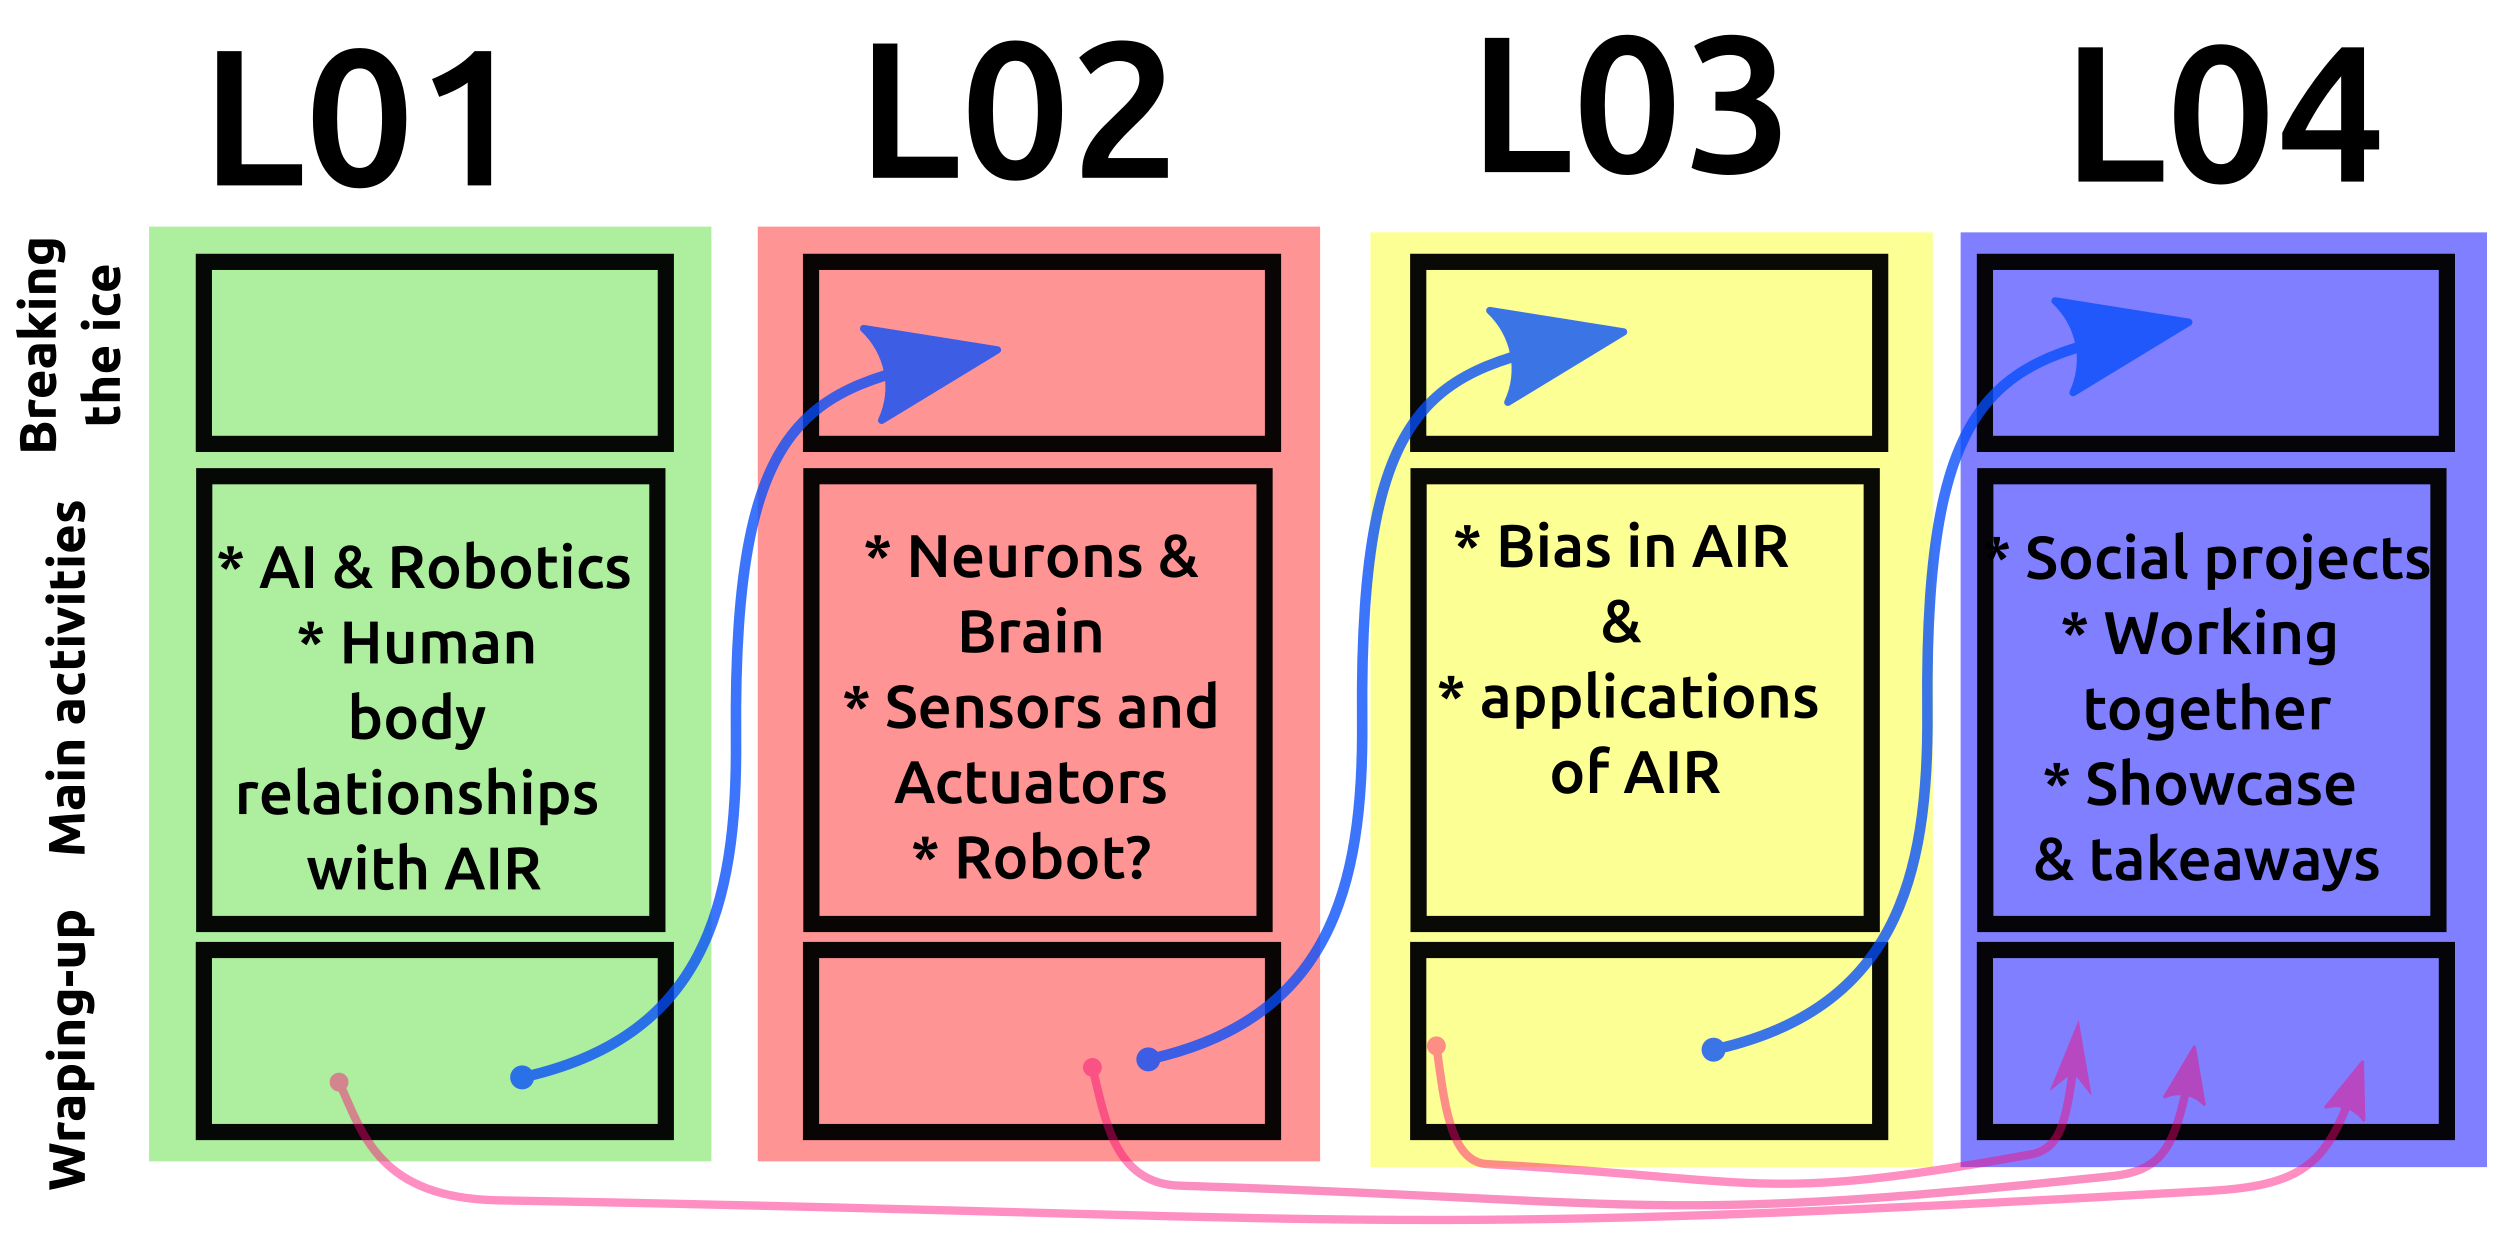
\includegraphics[width=1.0\textwidth]{./figures/curriculum/outputs/drawing-v00.png}
        %\caption{}
      \end{figure}
\end{frame}
}


%%%%%%%%%%%%%%%%%%%%%%%%%%%%%%%%%%%%%%%%%%%%%
\subsection{Piloting curriculum}

%%%%%%%%%%%%%%%%%%%%%%%%%%%%%%%%%%%%%%%%%%%%%%%%%%%%%%%%%
%{
%\paper{Badillo-Perez A, Badillo-Perez D, Barco A, Montenegro R, \textbf{Xochicale M. 2023}, Teaching AI and Robotics to Children in a Mexican town, DEI-HRI2023, \url{https://arxiv.org/abs/2303.03956}}
%
%\begin{frame}{Participants}
%
%\begin{itemize}
%\item 14 participants of which 10 were able to attend, 6 male and 4 female of (age in years: mean=8 and std=$\pm$1.61)     
%\item Four instructors of different teaching experience levels to young audiences.
%\end{itemize}
%
%\end{frame}
%}
%
%



%%%%%%%%%%%%%%%%%%%%%%%%%%%%%%%%%%%%%%%%%%%%%%%%%%%%%%%%
{

\paper{Badillo-Perez A, Badillo-Perez D, Barco A, Montenegro R, \textbf{Xochicale M. 2023}, Teaching AI and Robotics to Children in a Mexican town, DEI-HRI2023, \url{https://arxiv.org/abs/2303.03956}}

\begin{frame}{Piloting workshop: Coding and bingo activities}
      \begin{figure}
        \centering
        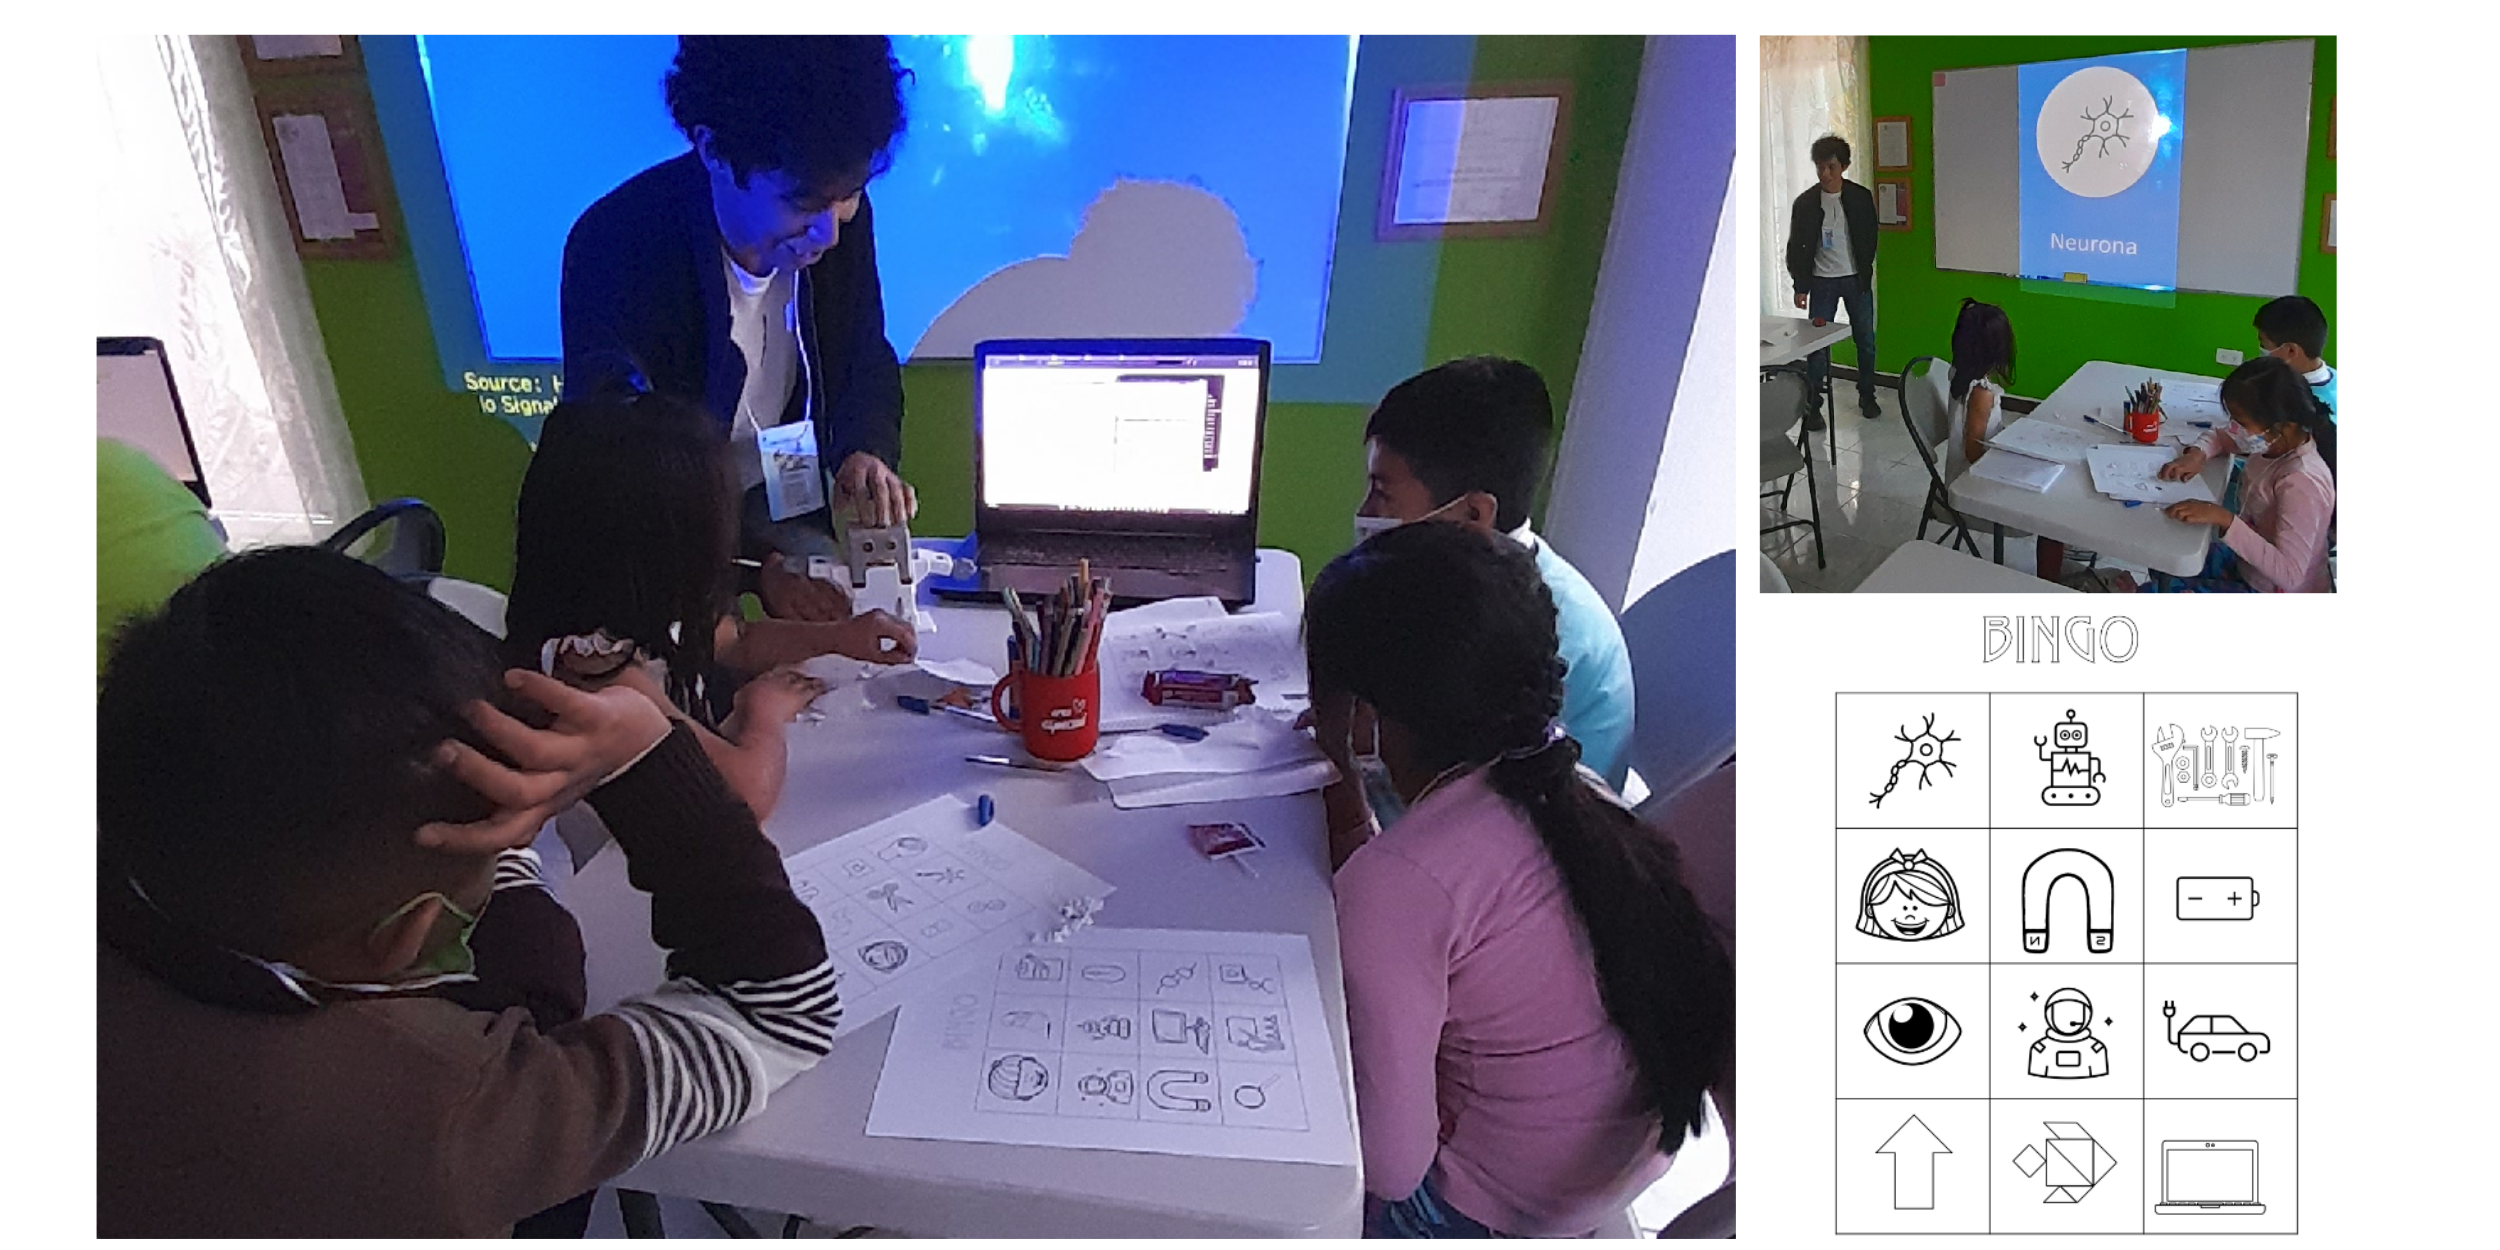
\includegraphics[width=1.0\textwidth]{./figures/pilot-workshop-a/outputs/drawing-v00.png}
        %\caption{}
      \end{figure}
\end{frame}
}



%%%%%%%%%%%%%%%%%%%%%%%%%%%%%%%%%%%%%%%%%%%%%%%%%%%%%%%%%
%{
%
%\paper{Badillo-Perez A, Badillo-Perez D, Barco A, Montenegro R, \textbf{Xochicale M. 2023}, Teaching AI and Robotics to Children in a Mexican town, DEI-HRI2023, \url{https://arxiv.org/abs/2303.03956}}
%
%\begin{frame}{Piloting workshop: Teaching activities}
%      \begin{figure}
%        \centering
%        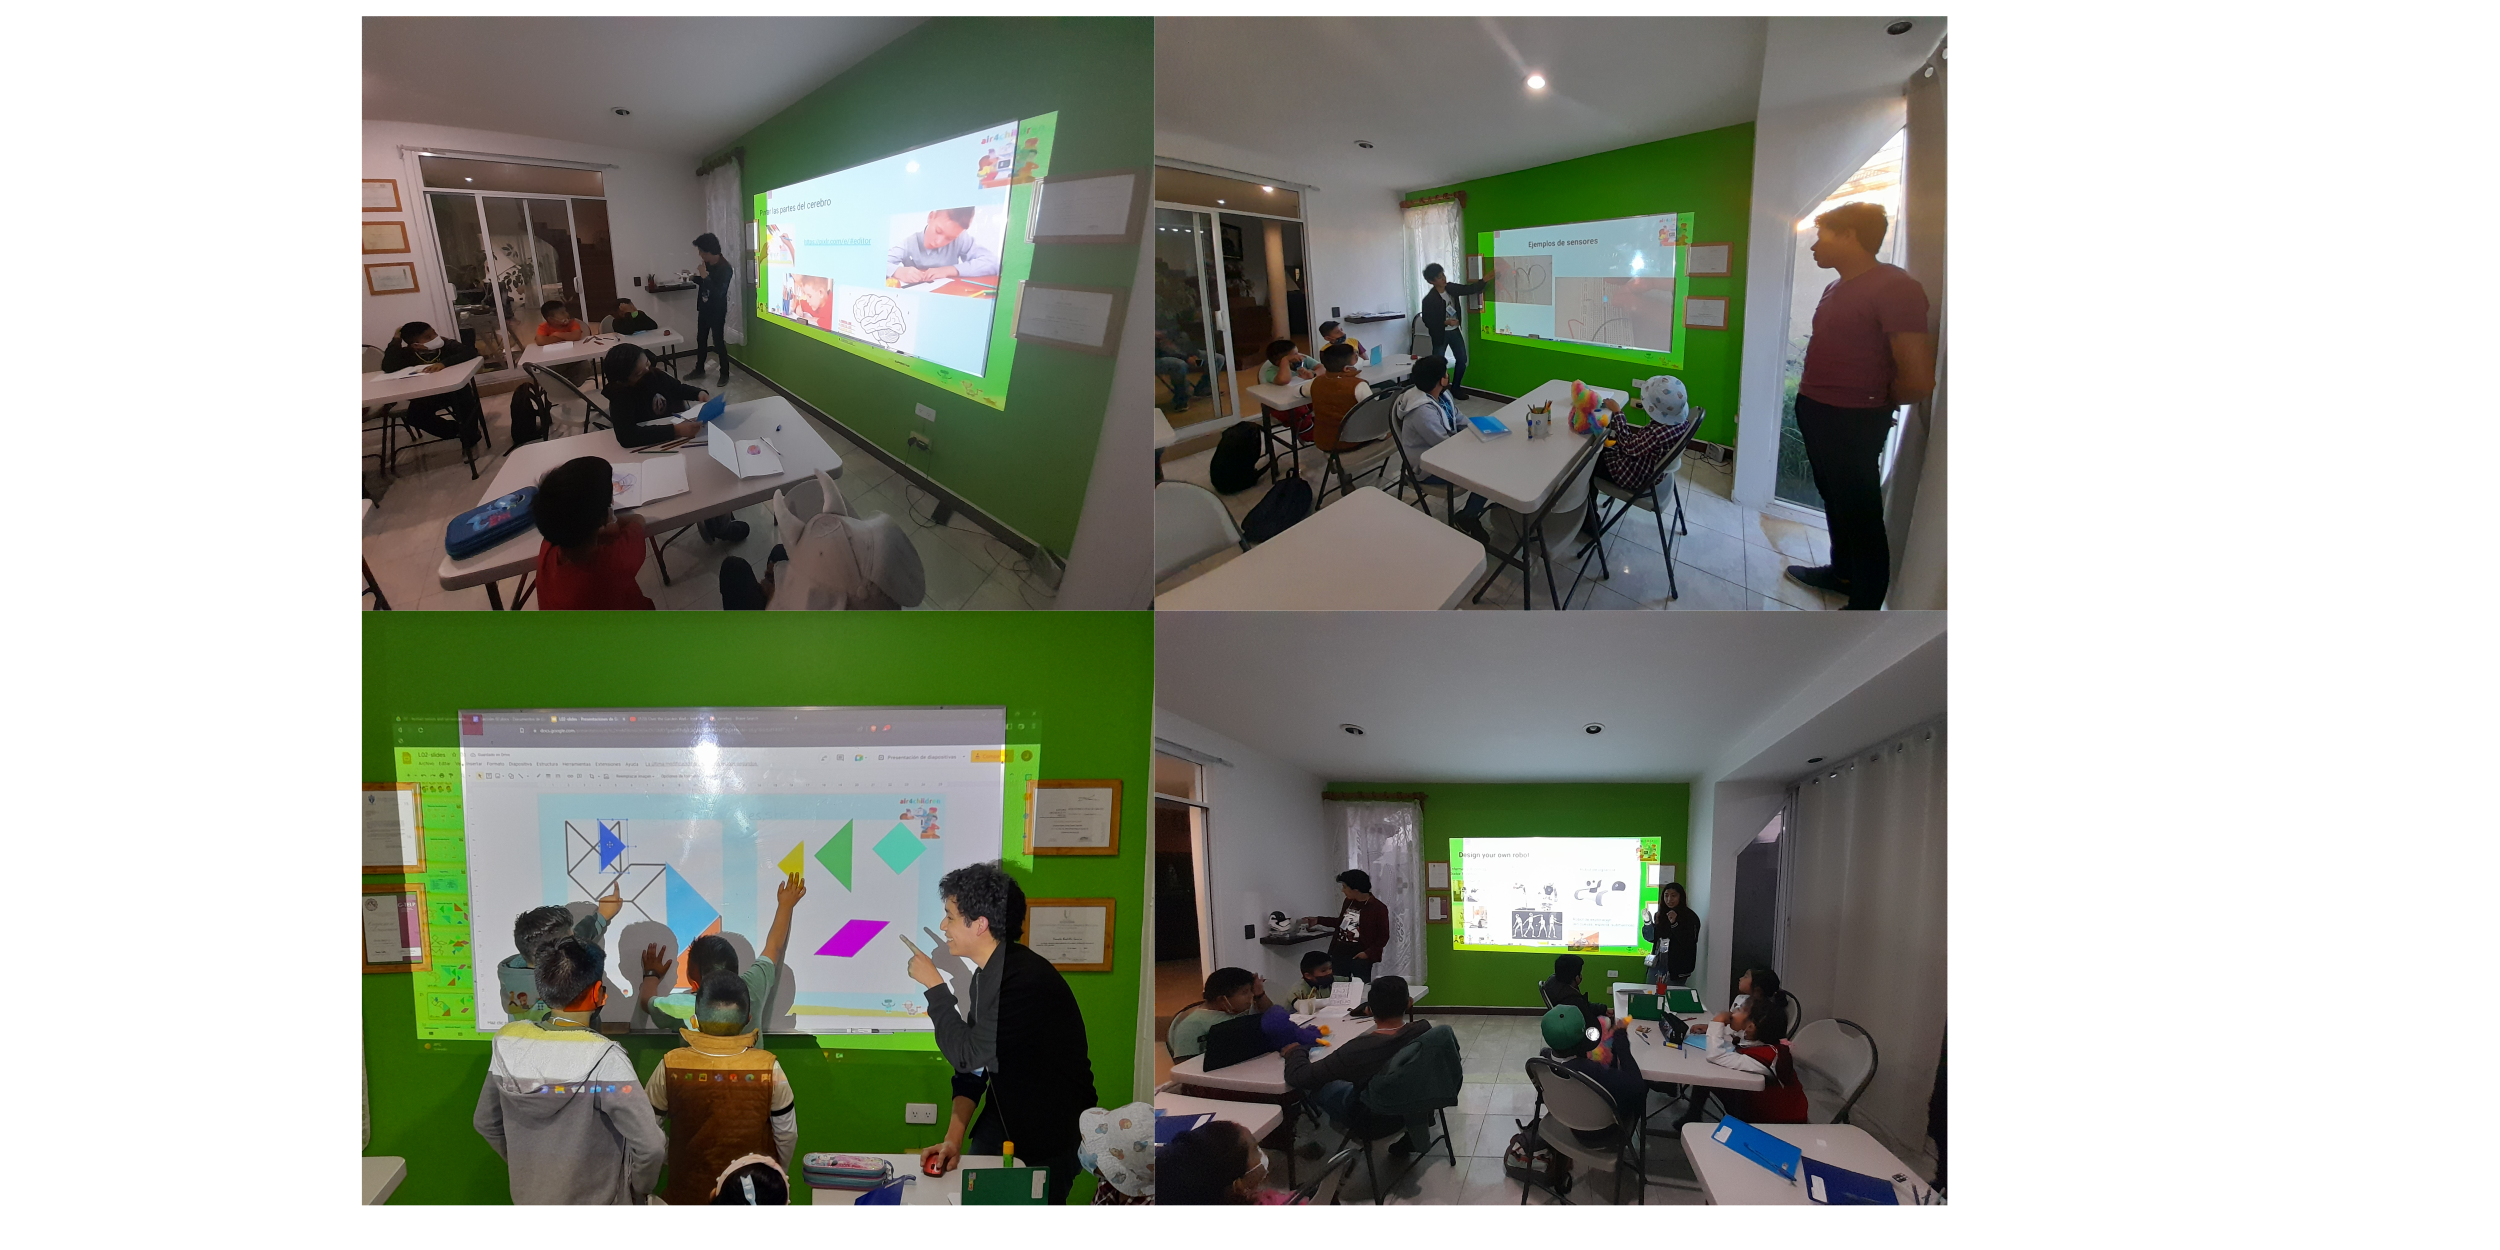
\includegraphics[width=1.0\textwidth]{./figures/pilot-workshop-b/outputs/drawing-v00.png}
%        %\caption{}
%      \end{figure}
%\end{frame}
%}
%

%%%%%%%%%%%%%%%%%%%%%%%%%%%%%%%%%%%%%%%%%%%%%%%%%%%%%%%%
{

\paper{Badillo-Perez A, Badillo-Perez D, Barco A, Montenegro R, \textbf{Xochicale M. 2023}, Teaching AI and Robotics to Children in a Mexican town, DEI-HRI2023, \url{https://arxiv.org/abs/2303.03956}}

\begin{frame}{Piloting workshop: Group activities}
      \begin{figure}
        \centering
        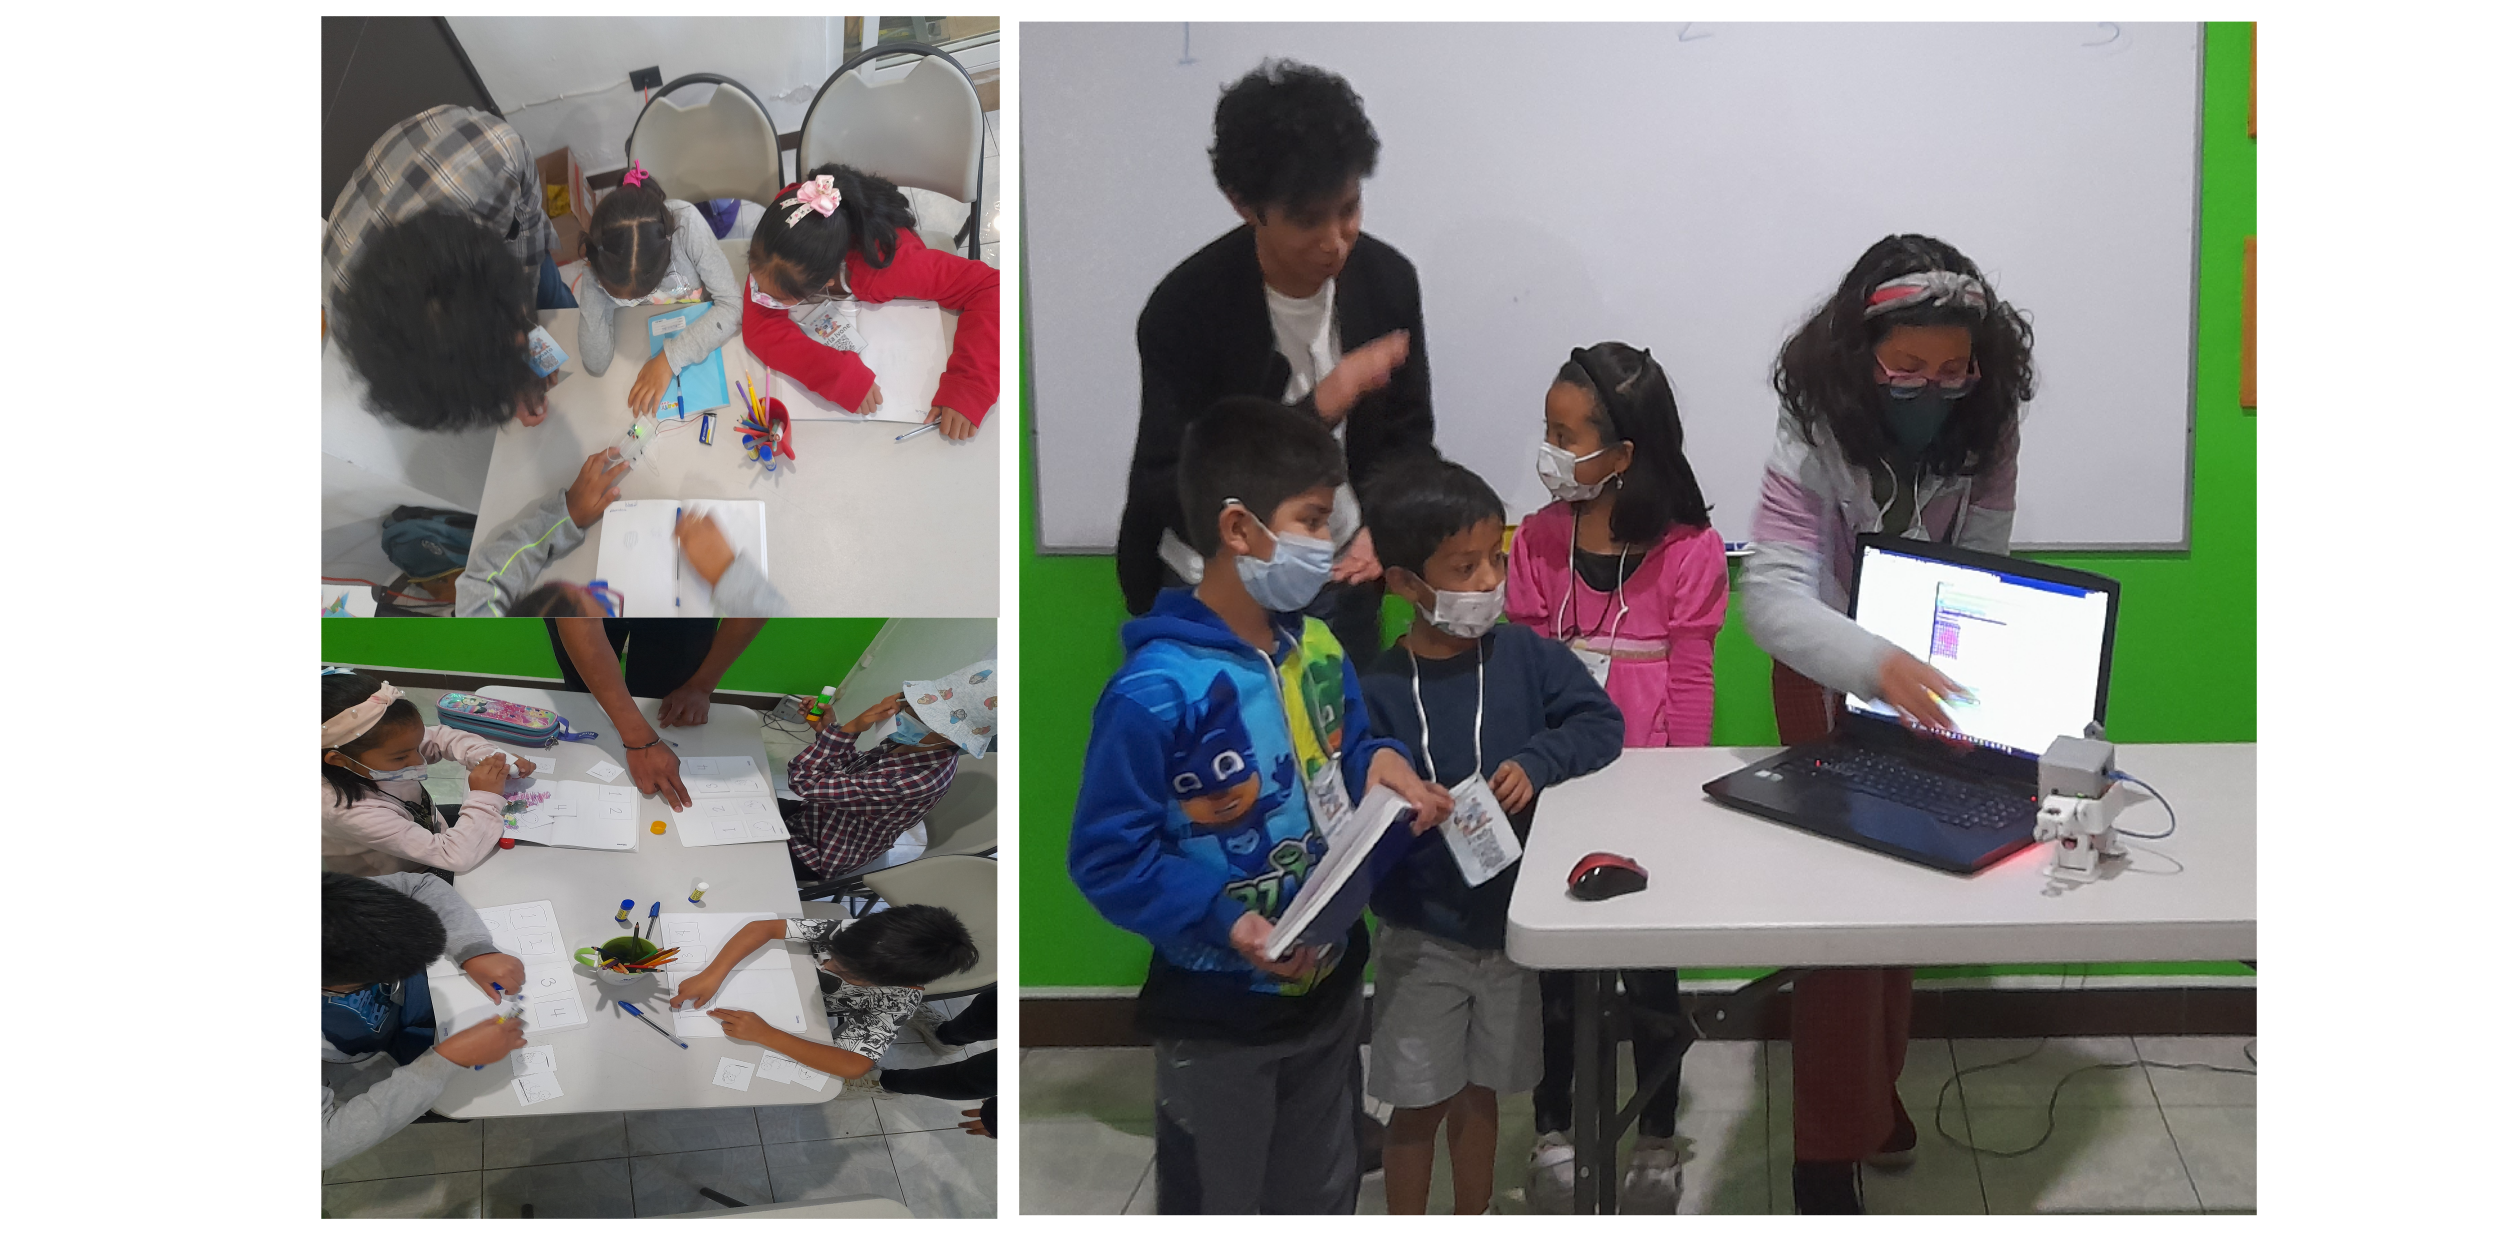
\includegraphics[width=1.0\textwidth]{./figures/pilot-workshop-c/outputs/drawing-v00.png}
        %\caption{}
      \end{figure}
\end{frame}
}

%%%%%%%%%%%%%%%%%%%%%%%%%%%%%%%%%%%%%%%%%%%%%
\subsection{Results of the survey}

%%%%%%%%%%%%%%%%%%%%%%%%%%%%%%%%%%%%%%%%%%%%%%%%%%%%%%%%
{

\paper{Badillo-Perez A, Badillo-Perez D, Barco A, Montenegro R, \textbf{Xochicale M. 2023}, Teaching AI and Robotics to Children in a Mexican town, DEI-HRI2023, \url{https://arxiv.org/abs/2303.03956}}

\begin{frame}{Survey results}
      \begin{figure}
        \centering
        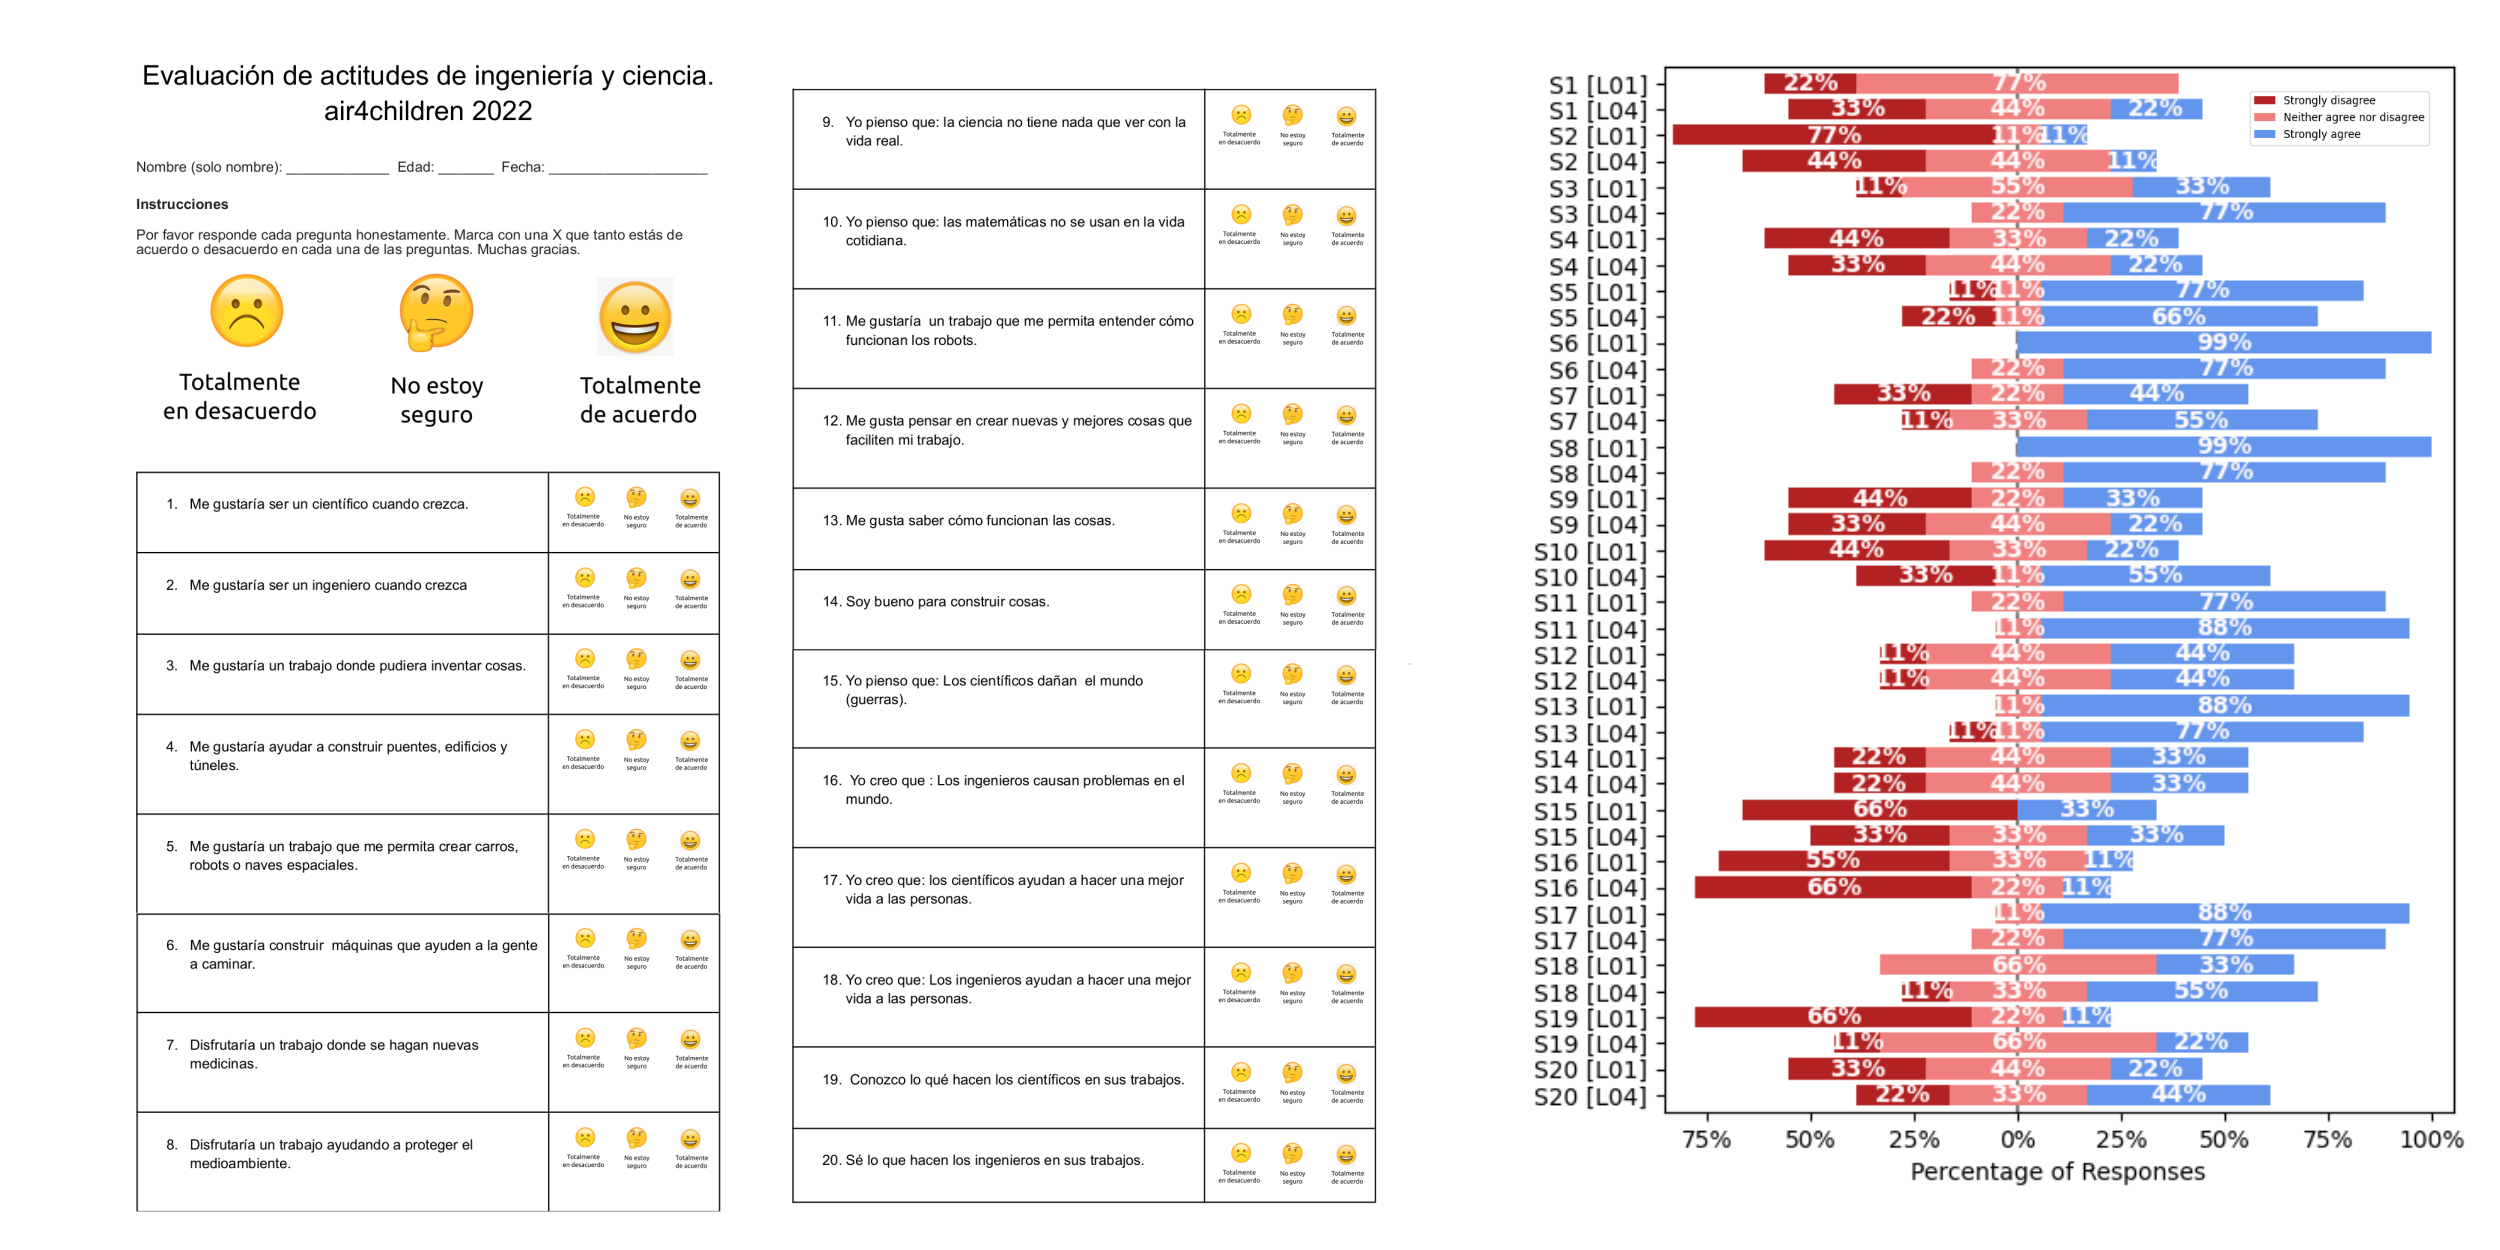
\includegraphics[width=1.0\textwidth]{./figures/survey-results/outputs/drawing-v00.png}
        %\caption{}
      \end{figure}
\end{frame}
}


%%%%%%%%%%%%%%%%%%%%%%%%%%%%%%%%%%%%%%%%%%%%%%%%%%%%%%%%%
%{
%\paper{Badillo-Perez A, Badillo-Perez D, Barco A, Montenegro R, \textbf{Xochicale M. 2023}, Teaching AI and Robotics to Children in a Mexican town, DEI-HRI2023, \url{https://arxiv.org/abs/2303.03956}}
%
%\begin{frame}{Statistical analysis}
%
%\begin{itemize}
%\item A Wilcoxon T test was used to analyze the results of the survey before and after the survey to see if the engineering attitudes had a significant effect on pre and post survey of the workshop.
%\item The average survey before the test was lower ($\mu$ = 2.194500 $\pm \sigma$ 0.558367 ) compared to the posttest results ($\mu$ = 2.239500 $\pm \sigma$= 0.396796).
%\item There was no statistically significant in the increase of attitudes towards engineering (t=53.5, p= 0.45).
%\end{itemize}
%
%See Appendix section for reproducible Jupyter notebooks of statistical analysis and plots.
%
%\end{frame}
%}
%


